\chapter{Opis projektnog zadatka}
		
%		\textbf{\textit{dio 1. revizije}}\\

	\section{Cilj i opis projekta na temelju dobivenog zadatka}	
	Cilj projekta je razviti web aplikaciju koja omogućuje dijeljenje recepata te tako pomaže korisnicima pri dijeljenju kulinarskih ideja, suradnji s drugim kreatorima recepata, organizaciji vlastite dijete i otkrivanju novih načina za pripremu jela. Tako korist od nje mogu imati profesionalni kuhari, nutricionisti, ali i kuhari amateri te osobe koje radi zdravstvenog stanja moraju prilagođavati dijetu. Novopridošlim korisnicima se prikazuju recepti sortirani od novijih prema starijima, što omogućuje da bez registracije imaju pregled kulinarskih trendova i odluče hoće li je nastaviti koristiti. Moguće se registrirati kao klijent, kuharski entuzijast ili nutricionist. Korisnik može administratorima poslati zahtjev za registraciju koji, jednom kad je odobren, dopušta korisniku da pretražuje profile i recepte na temelju dijete koju prate. Entuzijasti kreiraju recepte i kuharice, koje su skupovi recepata, dok nutricionisti kreiraju dijete koje nameću ograničenja na recepte. Korisnici neposredno prije kuhanja mogu unijeti prehrambeni artikl QR kodom ili izborom iz kataloga te tako filtrirati recepte u kojima se on nalazi. Tada se recepti sortiraju prema tome koliko dobro prate dijetu korisnika, odnosno koliko poštuju njena ograničenja. Korisnici također vide statistiku povijesti unosa nutritivnih vrijednosti. Što se implementacije tiče, aplikacija mora biti objektno orijentirana.

	\section{Potencijalna korist projekta}
	Osim očite koristi da korisnici među sobom dijele i objavljuju recepte i dijete, korist se može naći i u statistici unosa nutritivnih vrijednosti te vrstama recepata koju prate. Uzmimo u obzir da aplikacija \glqq zaživi\grqq, odnosno dostigne broj korisnika dovoljan da predstavlja državu ili neki njen dio. Tada bi vladajući mogli iskoristiti informaciju o tome što ljudi najviše jedu i subvencionirati domaće proizvođače tih proizvoda jer je njihova prodaja izglednija. S druge strane, mogli bi ciljati na raznolikost prehrane pa subvencionirati one koji proizvode hranu koja je u manjku. Profit tada nije tako izgledan kao u prvom slučaju, ali bi financijska motivacija navela proizvođače da se preusmjere te tako dođe do veće dostupnosti raznolike prehrane na tržištu. S obzirom da aplikacija vodi računa o preferencijama korisnika i dijetama koje odabiru, novi vlasnici restorana i drugih lokala koji poslužuju hranu bi mogli to iskoristiti da se specijaliziraju, odnosno nude proizvode u skladu s nekom dijetom. Kao što je naznačeno u rečenici prije, radilo bi se samo o preferencijama i dijetama, koje ne smatramo osobnim podatcima jer su to odabiri unutar aplikacije. Ljudi koji ne smiju konzumirati određene namirnice ili skupove namirnica radi zdravstvenog stanja ili uvjerenja ne mogu jesti u većini lokala. Podatci o dijetama i receptima koje korisnici vole omogućuju vlasnicima novih lokala da ponude takvim osobama obroke u obliku specijalnih menija ili pak specijaliziraju cijeli lokal za tu dijetu.

	\section{Slična, već postojeća rješenja}
	Kriteriji da rješenje smatramo sličnim:
	\begin{packed_item}
		\item Aplikacija/web mjesto mora biti forum, to jest mora imati mogućnost registriranja korisnika koji onda mogu raspravljati.
		\item Tema diskusije mora biti hrana.
		\item Mora postojati mogućnost filtriranja recepata prema više od jednog kriterija, ne nužno istovremeno.
	\end{packed_item}

		\subsection{kuhar.ba}
			\url{https://kuhar.ba} -- datum pristupa: 26.10.2023.
			Web mjesto na naslovnoj stranici ima mogućnost filtriranja recepata prema složenosti te kategorijama i grupama jela. Moguće se registrirati te potom dodavati recepte, komentirati ih te raspravljati na forumu. Recepti imaju fotografiju, popis sastojaka, detaljni opis koraka i oznake.
				\begin{figure}[H]
					\centering
					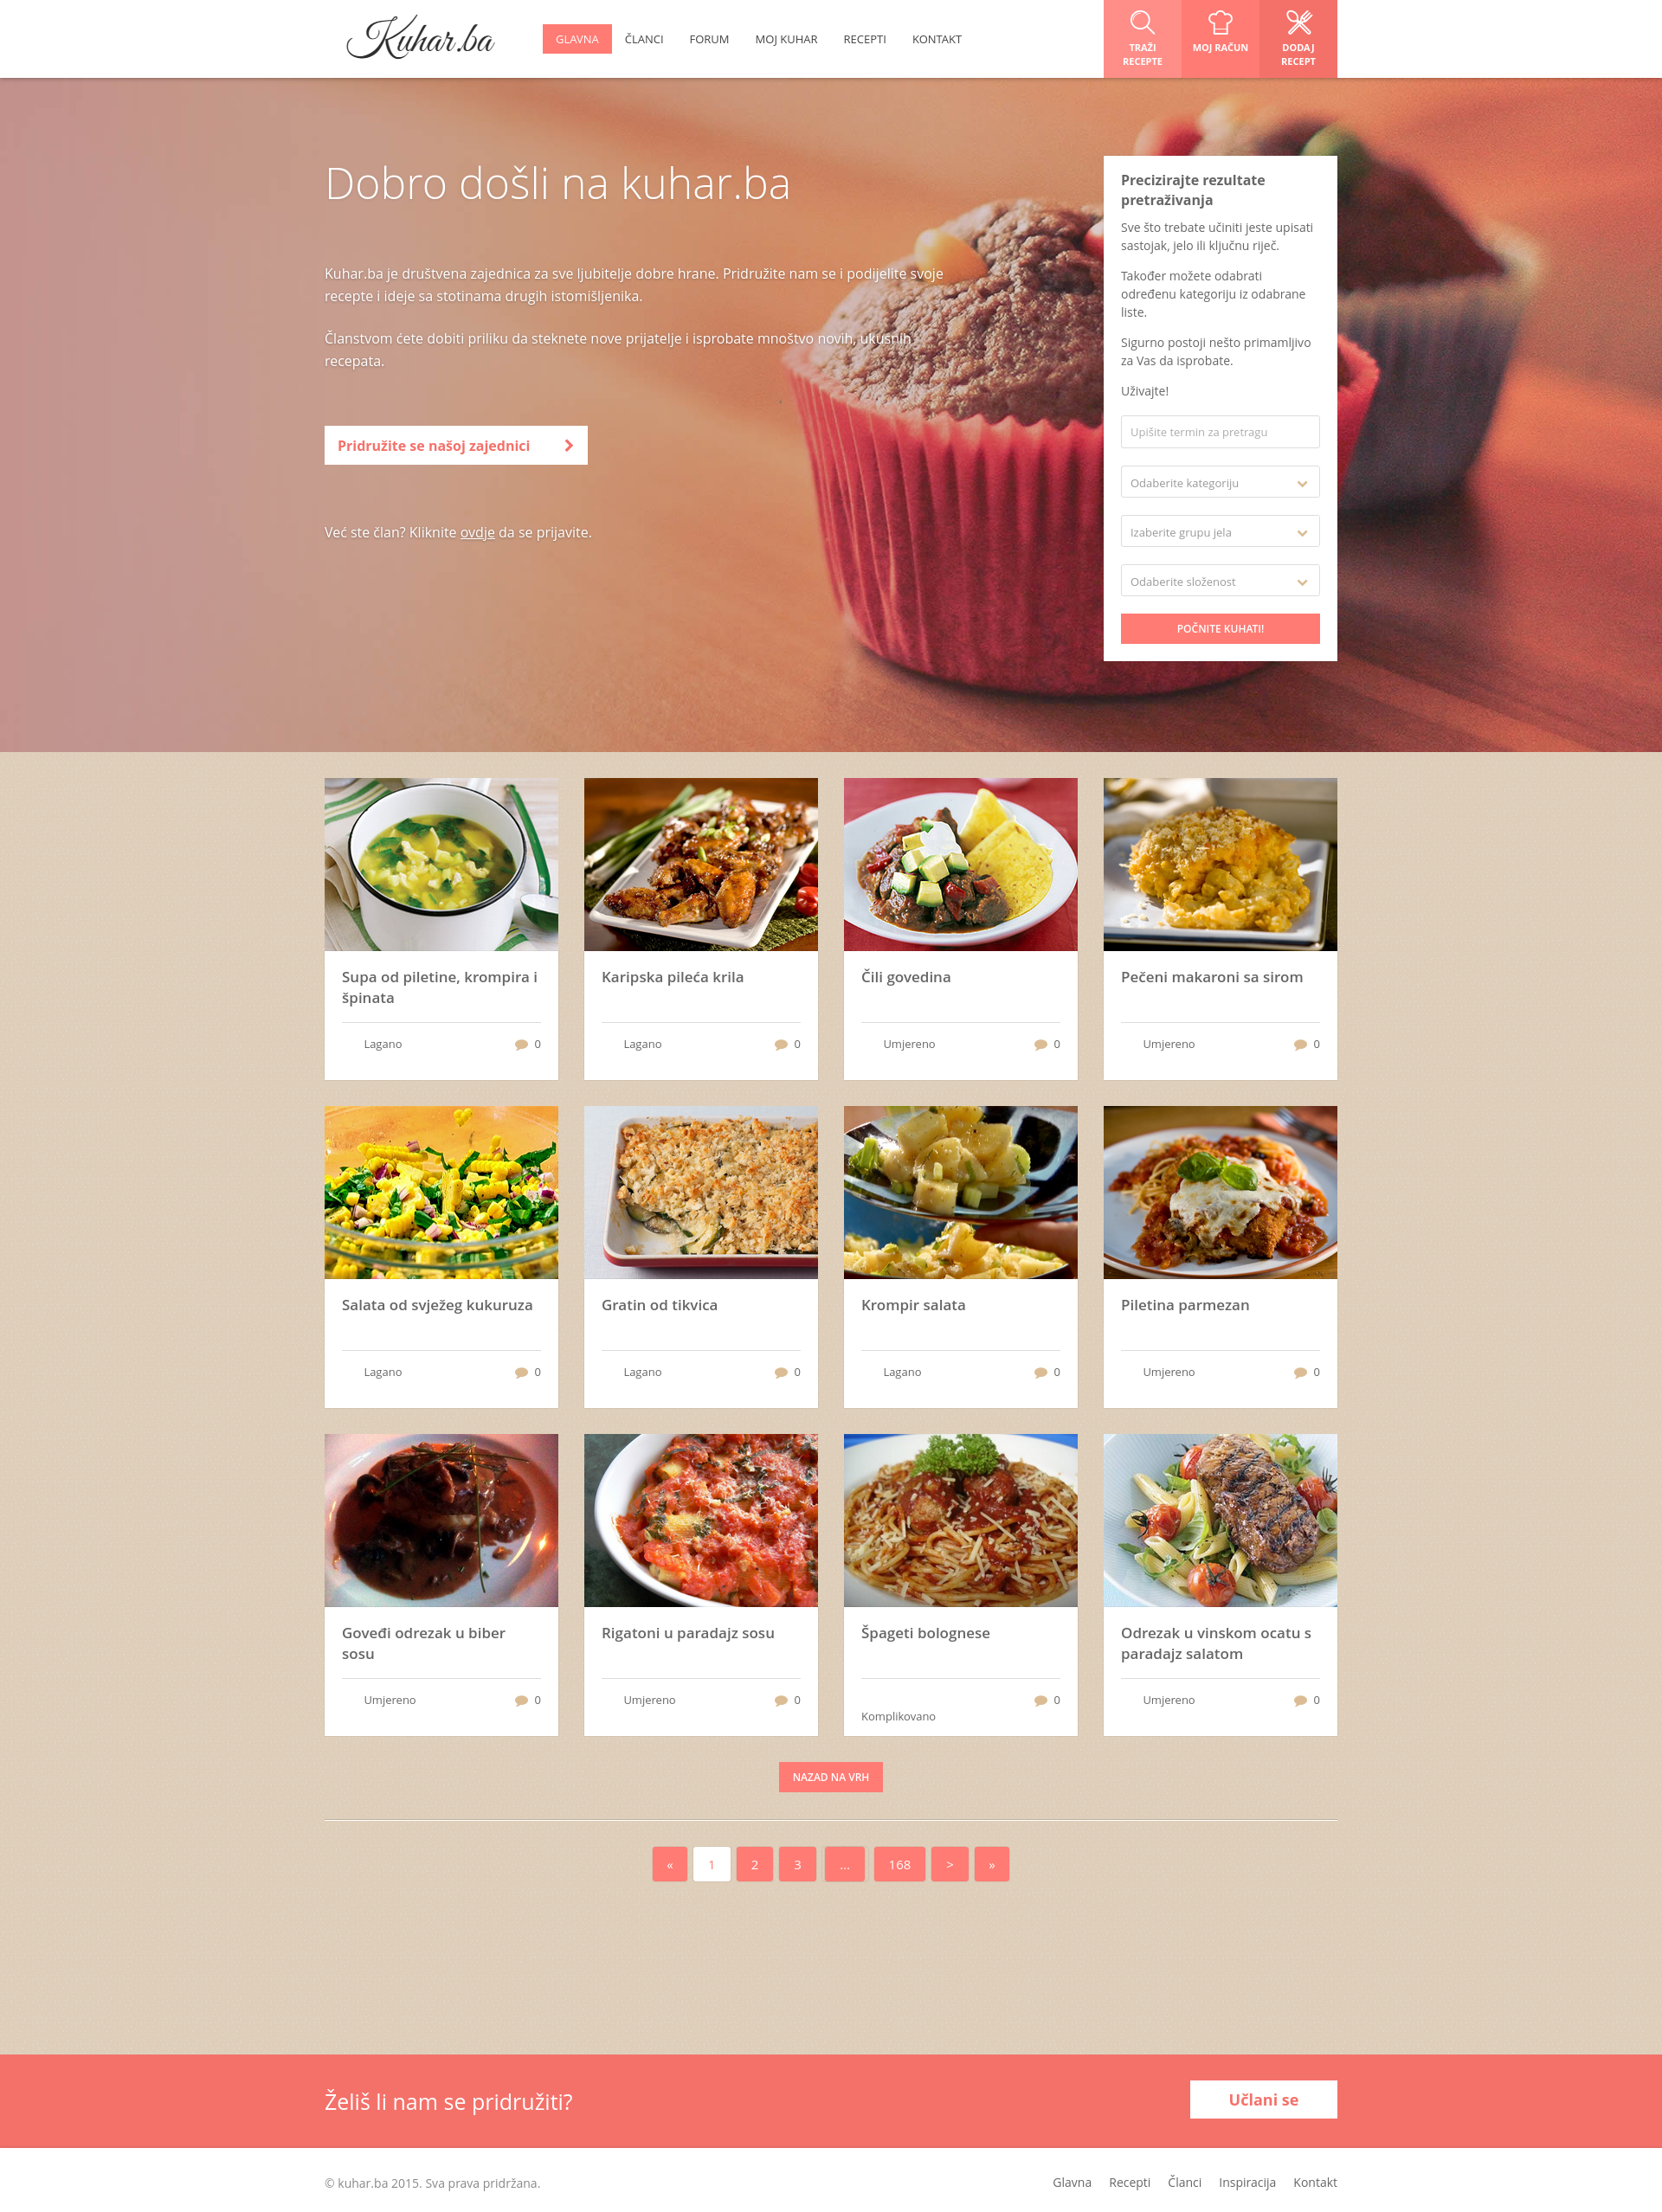
\includegraphics[scale=0.1]{slike/02-01-kuhar-ba.PNG}
					\caption{prednja strana web mjesta kuhar.ba}
					\label{fig:kuhar-ba-front}
				\end{figure} 
	

	\section{Skup korisnika koji bi mogao biti zainteresiran za ostvareno rješenje}
		\subsection {ako je aplikacija implementirana ovako}
		\begin{packed_item}
			\item kulinarski entuzijasti
			\item nutricionisti
			\item klijenti
			\item[]\begin{packed_item}
				\item profesionalni kuhari
				\item kuhari amateri
				\item osobe kojima je potrebna specijalna dijeta radi zdravstvenih razloga ili uvjerenja
			\end{packed_item}
		\end{packed_item}
		
		\subsection{ako je tematika aplikacije, u originalu kuhanje, to jest hrana prilagođena ciljanim korisnicima}
		\begin{packed_item}
			\item uradi sam majstori
			\item slikari
		\end{packed_item}
		Navedeni korisnici bi imali koristi od slične aplikacije. Općenitije, svaka zajednica ljudi za hobi ili zanimanje koje koristi algoritme, to jest radnje koje su podijeljene u niz koraka bi imalo koristi od slične aplikacije jer bi tako lakše razmjenjivali ideje i dolazili do inovacija u radu.

	\section{Mogućnost prilagodbe rješenja}
	Mana trenutnog rješenja je da ograničeno na objektno orijentirano pisanje jer to otežava skaliranje u budućnosti. Radi se o web (ili mobilnoj) aplikaciji koja treba imati sučelje koje je lako za razumjeti i koristi se u kuhinji, gdje, uz uobičajene laptope, mobitele i tablete, korisnici mogu imati i ostale pametne uređaje poput frižidera ili pećnica. Svi ti uređaji imaju web preglednik (ili operacijski sustav sličan Androidu ili nekoj konfiguraciji Linux-a) te su potencijalni klijenti. Što je više klijenata, baza podataka u pozadini je veća, a time i broj objekata, koji potiču problem upravljanja memorijom. Preporučeni programski jezici za poslužitelje, Java i Python uz Javascript, koji izvršavaju preglednici, svi redom koriste garbage collector. Činjenica je da taj proces šteti brzini rada aplikacije jer algoritam za "čišćenje" mora proći cijelu memoriju. Što više objekata, to više posla za taj algoritam pa stoga i veći period vremena koji sustav ili dijelovi sustava moraju provesti čekajući. Još k tomu niti dodavanje radne memorije ne pomaže jer to također algoritmu zadaje dodatan posao. Razumljivo je da se u vidu projekta na fakultetu objektno-orijentirana paradigma koristi u svrhu izrade dijagrama razreda (i drugih dijagrama, ali poglavito njega). Međutim, činjenica je da će takvo rješenje u upotrebi naići na probleme radi svega navedenog.

	\section{Opseg projektnog zadatka}
	Projekt obuhvaća:
	\begin{packed_item}
 		\item izradu web sučelja
		\item bazu podataka i komunikaciju s njom
		\item skeniranje QR kodova te njihovo generiranje
		\item izradu statističkog izvještaja na temelju podataka
	\end{packed_item}

	\section{Moguće nadogradnje projektnog zadatka}
		\subsection{Podržavanje hardverskog skenera kodova}
			S obzirom da aplikacija koristi kodove kao identifikator proizvoda, implementacija skeniranja hardverskim skenerom je moguća nadogradnja projektnog zadatka. Takvo rješenje bi zahtijevalo financijski trošak, ali bi poboljšalo rad aplikacije i olakšalo implementaciju. Umjesto "čupanja" koda iz datoteke sa slikom, uz gotov skener bi bilo dovoljno pročitati kod kao niz znakova na portu na korisničkom uređaju. To bi uzrokovalo znatno manju potrošnju mrežnog prometa i smanjilo vrijeme postavljanja koda na poslužitelj u usporedbi sa slikom. Također bi se rasteretio poslužitelj jer u tom slučaju nema potrebe za izvršavanjem algoritma za raspoznavanje koda iz slike.
	
		\subsection{Opcije za pristupačnost}
 			Korištenje aplikacije svodi se uglavnom na čitanje recepata. Stoga, bilo bi opravdano implementirati funkcionalnost korisničkog sučelja koja olakšava korištenje korisnicima koji imaju poteškoće s raspoznavanjem boja i slova. Dakle, riječ je o osobama s velikom dioptrijom, vrstama daltonizma i disleksijom. Kao funkcionalnost bi trebalo uvesti način rada u visokom kontrastu te mogućnost odabira fonta koji olakšava čitanje. Također bi bilo dobro implementirati pomični kursor kako bi se korisnik lakše orijentirao u tekstu. 

%		\textit{Na osnovi projektnog zadatka detaljno opisati korisničke zahtjeve. Što jasnije opisati cilj projektnog zadatka, razraditi problematiku zadatka, dodati nove aspekte problema i potencijalnih rješenja. Očekuje se minimalno 3, a poželjno 4-5 stranica opisa.	Teme koje treba dodatno razraditi u ovom poglavlju su:}
%		\begin{packed_item}
%			\item \textit{potencijalna korist ovog projekta}
%			\item \textit{postojeća slična rješenja (istražiti i ukratko opisati razlike u odnosu na zadani zadatak). Dodajte slike koja predočavaju slična rješenja.}
%			\item \textit{skup korisnika koji bi mogao biti zainteresiran za ostvareno rješenje.}
%			\item \textit{mogućnost prilagodbe rješenja }
%			\item \textit{opseg projektnog zadatka}
%			\item \textit{moguće nadogradnje projektnog zadatka}
%		\end{packed_item}
		
%		\textit{Za pomoć pogledati reference navedene u poglavlju „Popis literature“, a po potrebi konzultirati sadržaj na internetu koji nudi dobre smjernice u tom pogledu.}
%		\eject
%		
%		\section{Primjeri u \LaTeX u}
%		
%		\textit{Ovo potpoglavlje izbrisati.}\\
%
%		U nastavku se nalaze različiti primjeri kako koristiti osnovne funkcionalnosti \LaTeX a koje su potrebne za izradu dokumentacije. Za dodatnu pomoć obratiti se asistentu na projektu ili potražiti upute na sljedećim web sjedištima:
%		\begin{itemize}
%			\item Upute za izradu diplomskog rada u \LaTeX u - \url{https://www.fer.unizg.hr/_download/repository/LaTeX-upute.pdf}
%			\item \LaTeX\ projekt - \url{https://www.latex-project.org/help/}
%			\item StackExchange za Tex - \url{https://tex.stackexchange.com/}\\
%		
%		\end{itemize} 	


		
%		\noindent \underbar{podcrtani tekst}, \textbf{podebljani tekst}, 	\textit{nagnuti tekst}\\
%		\noindent \normalsize primjer \large primjer \Large primjer \LARGE {primjer} \huge {primjer} \Huge primjer \normalsize
%				
%		\begin{packed_item}
%			
%			\item  primjer
%			\item  primjer
%			\item  primjer
%			\item[] \begin{packed_enum}
%				\item primjer
%				\item[] \begin{packed_enum}
%					\item[1.a] primjer
%					\item[b] primjer
%				\end{packed_enum}
%				\item primjer
%			\end{packed_enum}
%			
%		\end{packed_item}
%		
%		\noindent primjer url-a: \url{https://www.fer.unizg.hr/predmet/proinz/projekt}
%		
%		\noindent posebni znakovi: \# \$ \% \& \{ \} \_ 
%		$|$ $<$ $>$ 
%		\^{} 
%		\~{} 
%		$\backslash$ 
%		
%		
%		\begin{longtblr}[
%			label=none,
%			entry=none
%			]{
%				width = \textwidth,
%				colspec={|X[8,l]|X[8, l]|X[16, l]|}, 
%				rowhead = 1,
%			} %definicija širine tablice, širine stupaca, poravnanje i broja redaka naslova tablice
%			\hline \SetCell[c=3]{c}{\textbf{naslov unutar tablice}}	 \\ \hline[3pt]
%			\SetCell{LightGreen}IDKorisnik & INT	&  	Lorem ipsum dolor sit amet, consectetur adipiscing elit, sed do eiusmod  	\\ \hline
%			korisnickoIme	& VARCHAR &   	\\ \hline 
%			email & VARCHAR &   \\ \hline 
%			ime & VARCHAR	&  		\\ \hline 
%			\SetCell{LightBlue} primjer	& VARCHAR &   	\\ \hline 
%		\end{longtblr}
%		
%
%		\begin{longtblr}[
%				caption = {Naslov s referencom izvan tablice},
%				entry = {Short Caption},
%			]{
%				width = \textwidth, 
%				colspec = {|X[8,l]|X[8,l]|X[16,l]|}, 
%				rowhead = 1,
%			}
%			\hline
%			\SetCell{LightGreen}IDKorisnik & INT	&  	Lorem ipsum dolor sit amet, consectetur adipiscing elit, sed do eiusmod  	\\ \hline
%			korisnickoIme	& VARCHAR &   	\\ \hline 
%			email & VARCHAR &   \\ \hline 
%			ime & VARCHAR	&  		\\ \hline 
%			\SetCell{LightBlue} primjer	& VARCHAR &   	\\ \hline 
%		\end{longtblr}
%	
%
%
%		
%		
%		%unos slike
%		\begin{figure}[H]
%			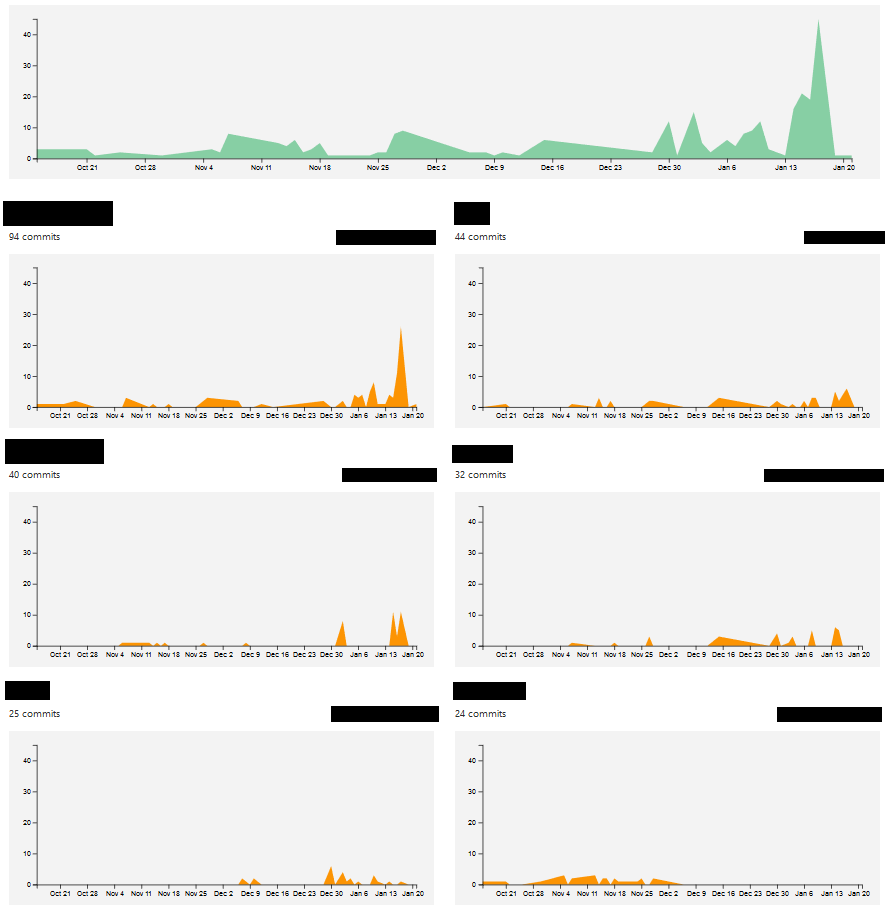
\includegraphics[scale=0.4]{slike/aktivnost.PNG} %veličina slike u odnosu na originalnu datoteku i pozicija slike
%			\centering
%			\caption{Primjer slike s potpisom}
%			\label{fig:promjene}
%		\end{figure}
%		
%		\begin{figure}[H]
%			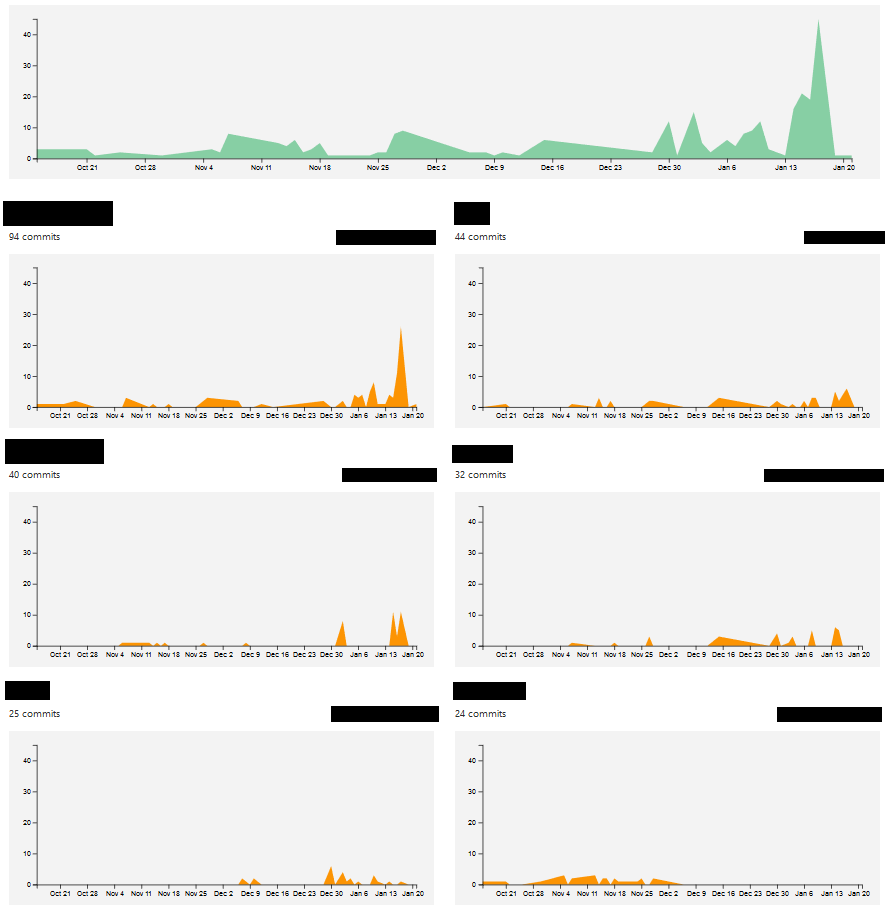
\includegraphics[width=\textwidth]{slike/aktivnost.PNG} %veličina u odnosu na širinu linije
%			\caption{Primjer slike s potpisom 2}
%			\label{fig:promjene2} %label mora biti drugaciji za svaku sliku
%		\end{figure}
%		
%		Referenciranje slike \ref{fig:promjene2} u tekstu.
%		
%		\eject
%		
	